\subsection{Uncertainties and Results}
\label{subsection: charged particle density, systematics}

\begin{figure}[h]
	\begin{subfigure}{0.49\textwidth}
		\includegraphics[width=\textwidth]{/afs/cern.ch/user/d/dvoong/cmtuser/DaVinci_v33r6/Phys/ChargedParticleMultiplicity/python/kinematic_distributions/tracks/systematics/data_files/TrackDistributionComparisonPlottingJob/bk/Down/real/-1/-1/pngs/eta_background_corrected_overlay.png}
		\caption{Background corrected charged particle density, $\eta$}
	\end{subfigure}
	\begin{subfigure}{0.49\textwidth}
		\includegraphics[width=\textwidth]{/afs/cern.ch/user/d/dvoong/cmtuser/DaVinci_v33r6/Phys/ChargedParticleMultiplicity/python/kinematic_distributions/tracks/systematics/data_files/TrackDistributionComparisonPlottingJob/bk/Down/real/-1/-1/pngs/eta_unfolded_overlay.png}
		\caption{Unfolded charged particle density, $\eta$}
	\end{subfigure}
	\begin{subfigure}{0.49\textwidth}
		\includegraphics[width=\textwidth]{/afs/cern.ch/user/d/dvoong/cmtuser/DaVinci_v33r6/Phys/ChargedParticleMultiplicity/python/kinematic_distributions/tracks/systematics/data_files/TrackDistributionComparisonPlottingJob/bk/Down/real/-1/-1/pngs/pt_background_corrected_overlay.png}
		\caption{Background  charged particle density, $p_\mathrm{T}$}
	\end{subfigure}
	\begin{subfigure}{0.49\textwidth}
		\includegraphics[width=\textwidth]{/afs/cern.ch/user/d/dvoong/cmtuser/DaVinci_v33r6/Phys/ChargedParticleMultiplicity/python/kinematic_distributions/tracks/systematics/data_files/TrackDistributionComparisonPlottingJob/bk/Down/real/-1/-1/pngs/pt_unfolded_overlay.png}
		\caption{Unfolded charged particle density, $p_\mathrm{T}$}
	\end{subfigure}
	\caption{Uncertainty of the corrected charged particle density in measured data due to statistical errors in the purity and efficiency}
	\label{fig: statistical uncertainty of corrected charged particle density, measured data}
\end{figure}

Since the purity and efficiency distributions are calculated from MC generated data, there is an associated uncertainty due to the statistical error in their distributions. This uncertainty is estimated by applying the correction procedure with the values of the purity and efficiency varied by their standard deviation. The resulting corrected distributions are shown in figure \ref{fig: statistical uncertainty of corrected charged particle density, measured data} for measured data and figure \ref{fig: statistical uncertainty of corrected charged particle density, mc data} for MC data.

\begin{figure}[h]
	\begin{subfigure}{0.49\textwidth}
		\includegraphics[width=\textwidth]{/afs/cern.ch/user/d/dvoong/cmtuser/DaVinci_v33r6/Phys/ChargedParticleMultiplicity/python/kinematic_distributions/tracks/systematics/data_files/TrackDistributionComparisonPlottingJob/bk/Down/mc/-1/-1/pngs/eta_background_corrected_overlay.png}
		\caption{Background corrected charged particle density, $\eta$}
	\end{subfigure}
	\begin{subfigure}{0.49\textwidth}
		\includegraphics[width=\textwidth]{/afs/cern.ch/user/d/dvoong/cmtuser/DaVinci_v33r6/Phys/ChargedParticleMultiplicity/python/kinematic_distributions/tracks/systematics/data_files/TrackDistributionComparisonPlottingJob/bk/Down/mc/-1/-1/pngs/eta_unfolded_overlay.png}
		\caption{Unfolded charged particle density, $\eta$}
	\end{subfigure}
	\begin{subfigure}{0.49\textwidth}
		\includegraphics[width=\textwidth]{/afs/cern.ch/user/d/dvoong/cmtuser/DaVinci_v33r6/Phys/ChargedParticleMultiplicity/python/kinematic_distributions/tracks/systematics/data_files/TrackDistributionComparisonPlottingJob/bk/Down/mc/-1/-1/pngs/pt_background_corrected_overlay.png}
		\caption{Background  charged particle density, $p_\mathrm{T}$}
	\end{subfigure}
	\begin{subfigure}{0.49\textwidth}
		\includegraphics[width=\textwidth]{/afs/cern.ch/user/d/dvoong/cmtuser/DaVinci_v33r6/Phys/ChargedParticleMultiplicity/python/kinematic_distributions/tracks/systematics/data_files/TrackDistributionComparisonPlottingJob/bk/Down/mc/-1/-1/pngs/pt_unfolded_overlay.png}
		\caption{Unfolded charged particle density, $p_\mathrm{T}$}
	\end{subfigure}
	\caption{Uncertainty of the corrected charged particle density in MC data due to statistical errors in the purity and efficiency}
	\label{fig: statistical uncertainty of corrected charged particle density, mc data}
\end{figure}

The uncertainty in the background correction of the charged particle density is dominated by the ghost correction, this can been seen in figure \ref{fig: background rates}. The systematic error on the ghost estimation is estimated by comparing the ghost rates calculated in section \ref{subsection: charged particle density, background corrected distributions} to a data driven method of ghost estimation. 

From MC data it can be seen that the dominant source of ghost tracks is from mis-matching VELO track segments (see section \ref{subsection: tracking, track reconstruction}) to hits or track segments in the T-stations - these hits may be due to other particles or detector noise. The data driven method of estimates these effects using the VELO flip method; this involves taking a reconstructed VELO track segment and flipping its direction in x and y. The flipped VELO track segment is then used as a seed in the forward track matching reconstruction algorithm that attempts to match the segment to hits or other track segments in the T-stations. Forward tracks reconstructed using the flipped VELO segment as its seed are then classified as ghost tracks.

In order for the track to be reconstructed it must meet several criteria such as a quality of fit ($\chi^2$) cut. In addition to this the track must be a better candidate than other combinations of the VELO track segment seed and T-station hits or track segments. In order to make an accurate estimation of the ghost rate the track candidates from the flipped VELO track segment are compared to the candidates from the original VELO track segment, if the best track candidate is from the flipped VELO track segment then it is kept.

\begin{figure}[h]
	\centering
	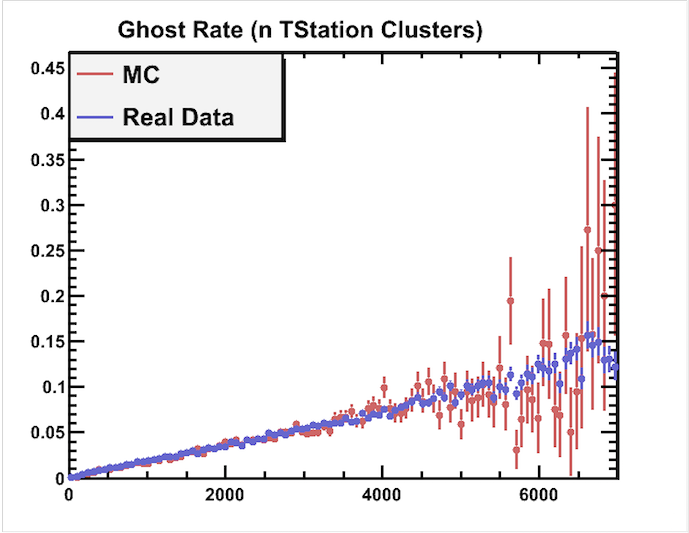
\includegraphics[width=0.49\textwidth]{Chapters/multiplicity/images/ghost_rate_data_driven.png}
	\caption{Ghost rates as a function of T-station hit multiplicity calculated using the data driven VELO flip method. The data points in red correspond to the ghost rate in MC data and the blue data points correspond to measured data. A good agreement is present between MC and measured data.}
	\label{fig: ghost rates, velo flip}
\end{figure}

Due to the nature of the matching algorithm, events with higher activity (expressed by the number of hits in the T-stations) in the detector are expected to have higher ghost rates. The ghost rate is plotted as a function of the T-station multiplicity (figure \ref{fig: ghost rates, velo flip}). The ghost rate is determined by the ratio of ghost classified tracks to the number of VELO track segments in an event, to translate this to the context of long tracks used in this analysis the ghost rate in long tracks is related to the ghost rate in VELO tracks scaled by the ratio of VELO tracks to long tracks. 

\begin{equation}
	R_\mathrm{long} = R_\mathrm{VELO} \cdot \frac{n_\mathrm{VELO}}{n_\mathrm{long}}
\end{equation}

where $R_\mathrm{long}$ is the ghost rate in long tracks, $R_\mathrm{VELO}$ is the ghost rate in VELO tracks, $n_\mathrm{VELO}$ is the number of velo tracks and $n_\mathrm{long}$ is the number of long tracks in the event. The overall ghost rate is then calculated from the average of the ghost rate in all events. The comparison between ghost rate estimation using the VELO flip method is shown in figure \ref{fig: ghost rates, velo flip}; there is good agreement between measured and MC data. A conservative estimate of 2\% for the systematic error was made for this analysis, as is the case for similar analyses such as \cite{Aaij:1662427}.

The final results for the charged particle density are shown in figure \ref{fig: corrected charged particle densities} with the systematics errors shown by the blue shaded boxes. A comparison between the unfolded distribution and charged particle distributions in MC generated events are shown for several event generators in figure \ref{fig: corrected charged particle densities, comparison}. 

\begin{figure}[h]
	\centering
	\begin{subfigure}{0.49\textwidth}
		\includegraphics[width=\textwidth]{/afs/cern.ch/user/d/dvoong/cmtuser/DaVinci_v33r6/Phys/ChargedParticleMultiplicity/python/kinematic_distributions/tracks/results/data_files/manual/real/eta.png}
		\caption{$\eta$}
		\label{fig: charged particle density, eta result}
	\end{subfigure}
	\begin{subfigure}{0.49\textwidth}
		\includegraphics[width=\textwidth]{/afs/cern.ch/user/d/dvoong/cmtuser/DaVinci_v33r6/Phys/ChargedParticleMultiplicity/python/kinematic_distributions/tracks/results/data_files/manual/real/pt.png}
		\caption{$p_\mathrm{T}$}
		\label{fig: charged particle density, pt result}
	\end{subfigure}
	\caption{Corrected charged particle densities, systematic errors are shown by the shaded blue areas}
	\label{fig: corrected charged particle densities}
\end{figure}

\begin{figure}[H]
	\centering
	\begin{subfigure}{0.49\textwidth}
		\includegraphics[width=\textwidth]{/afs/cern.ch/user/d/dvoong/cmtuser/DaVinci_v33r6/Phys/ChargedParticleMultiplicity/python/kinematic_distributions/tracks/results/data_files/manual/real/eta_comparison.png}
		\caption{$\eta$}
		\label{fig: charged particle density, eta result}
	\end{subfigure}
	\begin{subfigure}{0.49\textwidth}
		\includegraphics[width=\textwidth]{/afs/cern.ch/user/d/dvoong/cmtuser/DaVinci_v33r6/Phys/ChargedParticleMultiplicity/python/kinematic_distributions/tracks/results/data_files/manual/real/pt_comparison.png}
		\caption{$p_\mathrm{T}$}
		\label{fig: charged particle density, pt result}
	\end{subfigure}
	\caption{Comparison of corrected charged particle densities between measured data and several MC generators.}
	\label{fig: corrected charged particle densities, comparison}
\end{figure}
